\chapter{Results}

The results include three parts of the study. 
First, the performance of rCOMMIT on different subsets will be visualized and the pseudo ground truth based on 
rCOMMIT is summarized for each subject.
Second, the performance of the deep learning models trained on the pseudo ground truth will be shown. 
As mentioned, similar study has been conducted with SIFT \cite{smithSIFTSphericaldeconvolutionInformed2013} on the same subjects.
Last, this study makes a comparison between COMMIT and SIFT about the filtering results and the model performance. 

\section{Performance of rCOMMIT}

Fig. \ref{fig:ARplot} and Fig. \ref{fig:heatmap} show the distribution of ARs in different subset sizes on three subjects, 
and table \ref{table:cate} indicates the values and the ranges of categories. 
Summing up the proportion in category 0 and 6, the result shows that more than 50\% of the streamlines
are of either 0\% AR or 100\% AR after running rCOMMIT for all the subsets. For the tractograms of 10 million streamlines, all the streamlines
are divided into category 0 and 6. 
Besides, the filtering results from this size of tractograms are consistent.

When applying COMMIT to the smaller datasets, the proportion of streamlines from 
category 1 to 5 increases. Meanwhile, the proportion of streamlines with AR = 100\% increases from 7.0\% to 28.5\%,
while the proportion of streamlines with AR = 0\% decreases largely, from 93.4\% to 27.2\%.
The relationship between the ARs and the length is also analyzed in Fig. \ref{fig:ARplot}, which shows the same trends as Fig. \ref{fig:heatmap}.


\begin{table}[!ht]
    \centering
    \caption{The values and ranges of different acceptance rate categories. For category 0, the AR is 0\%.
         For category 6, the AR is 100\%. For the other categories, the ARs are classified by the ranges. These intervals 
         do not include the lower bound and include the higher bound, except category 5 which excludes both 80\% and 100\%.}
    ~\\
    \label{table:cate}
    \begin{tabular}{p{5cm} p{5cm}}
    \toprule
    \textbf{Category}		  & \textbf{Acceptance Rate(AR)}\\
    \hline
    0                   & 0\% \\
    \hline
    1                   & (0\%,20\%{]} \\
    \hline
    2                 & (20\%,40{]} \\
    \hline
    3                 & (40\%,60\%{]} \\
    \hline
    4                 & (60\%,80\%{]} \\
    \hline 
    5                 & (80\%,100\%) \\
    \hline
    6                 & 100\% \\
    \bottomrule
    \end{tabular}
\end{table}

\begin{figure}[ht]
    \centering
    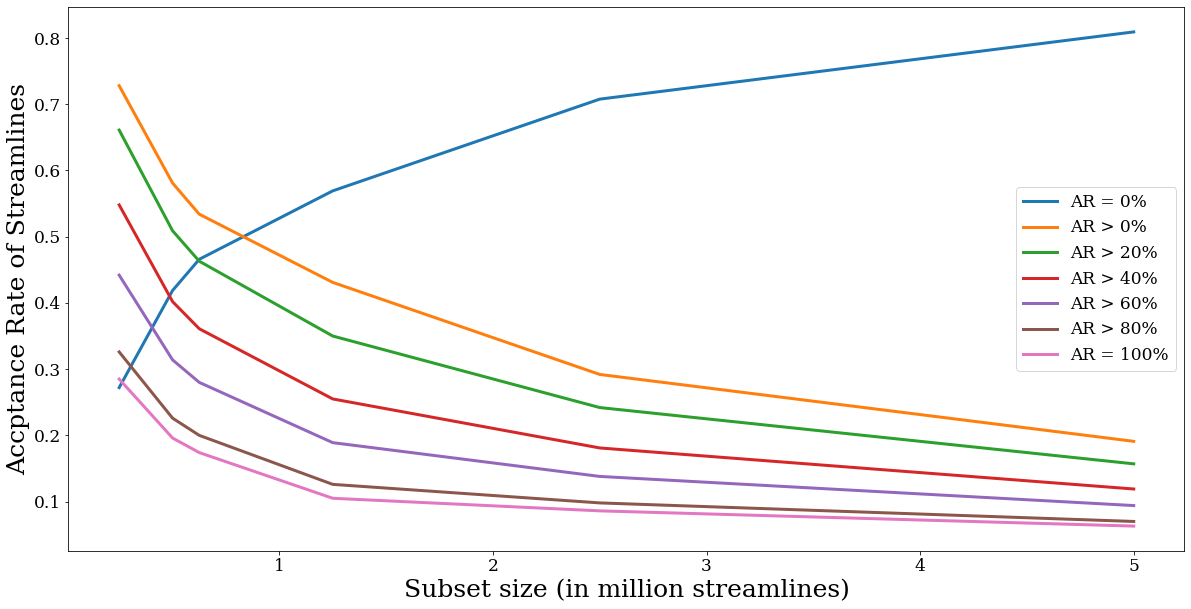
\includegraphics[width= 12cm]{figures/ARplot.png}
        \caption{The changes of acceptance rate from rCOMMIT with different subset size.
        The curves show the averaged AR over subjects. As shown, the ARs of streamlines get higher in the smaller
        subsets.}
    \label{fig:ARplot}
\end{figure}

\begin{figure}[ht]
    \centering
    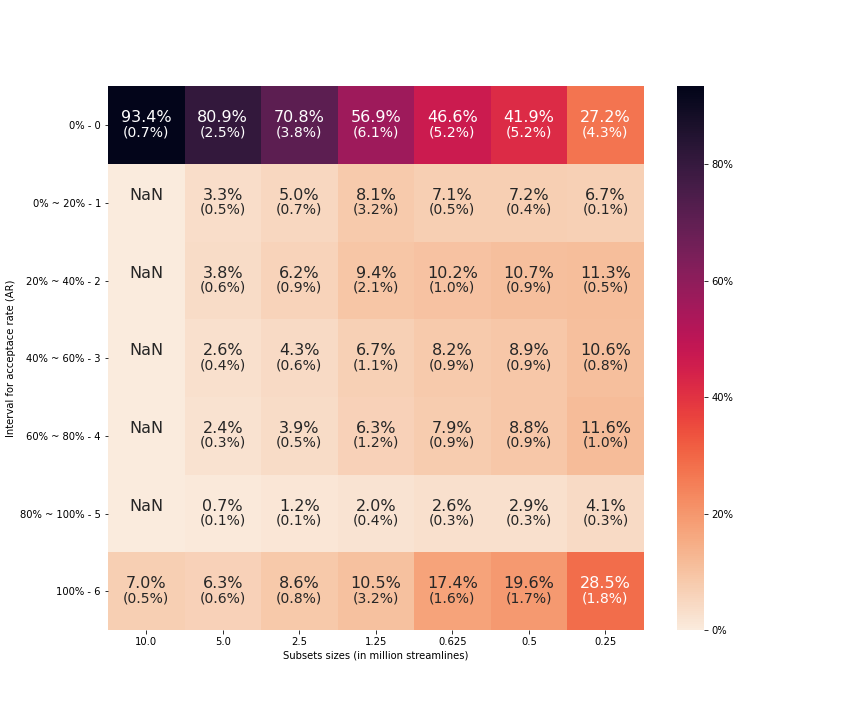
\includegraphics[width= 12cm]{figures/heatmap_new.png}
        \caption{The distribution of acceptance rates in different subset sizes. Each cell includes the mean ratio of 
        the streamlines across subjects and the standard deviations in the parentheses. In the column of the 10 million data, there is no value from category 1 to 5.
        }
    \label{fig:heatmap}
\end{figure}

The distribution of results between normal COMMIT and rCOMMIT are shown in Fig. \ref{fig:ori_distri} and Fig. \ref{fig:threegroup}.
As shown in the Fig. \ref{fig:ori_distri}, only a small amount of streamlines is kept by COMMIT. As shown in the Fig. \ref{fig:threegroup}, the rCOMMIT influences the distribution of the streamlines and the remaining 
streamlines are mostly among the short ones. The length of rejected streamlines is of higher variety. The distribution of inconclusive streamlines
is similar to the distribution of the input data.

\begin{figure}[ht]
    \centering
    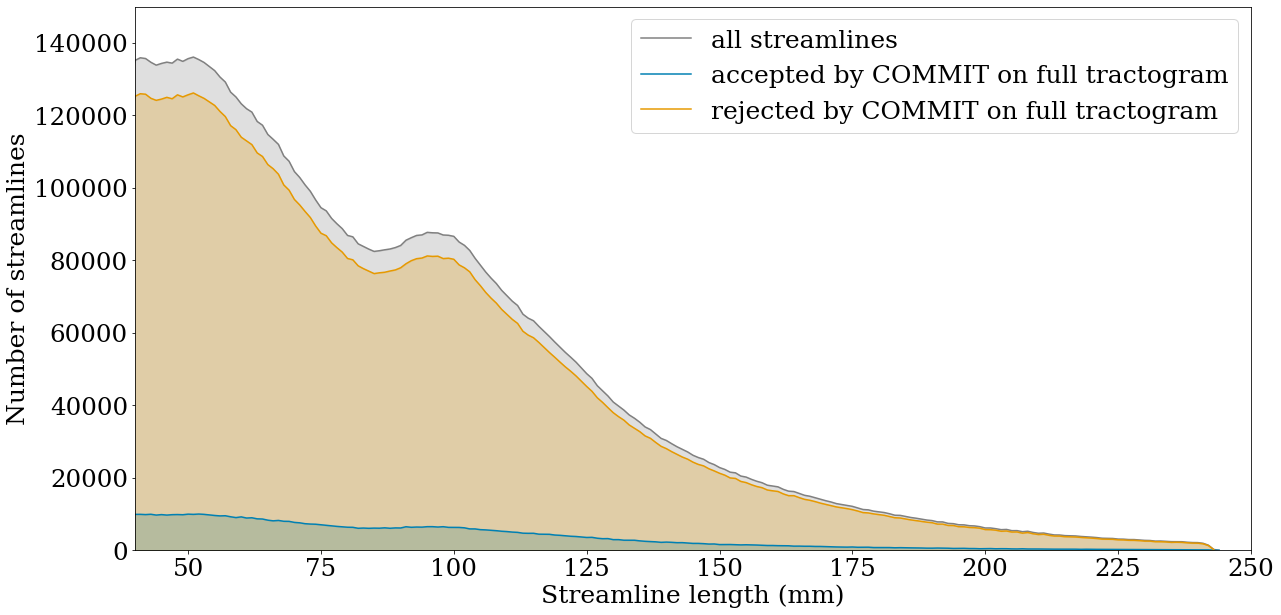
\includegraphics[width= 12cm]{figures/distributon_origi.png}
        \caption{The distribution of streamlines from one exemplary subject filtered by COMMIT. COMMIT is applied on the raw data of 10 million streamlines, which are 
        divided into two groups: rejected and accepted groups.}
    \label{fig:ori_distri}
\end{figure}

\begin{figure}[ht]
    \centering
    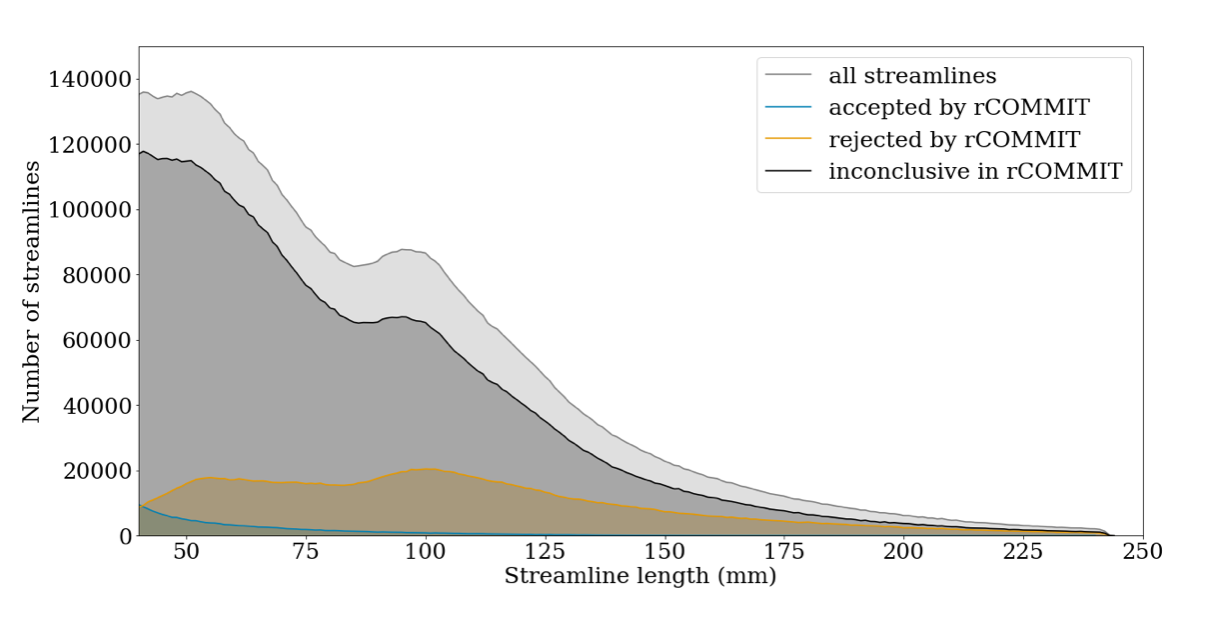
\includegraphics[width= 12cm]{figures/three_groups_hist.png}
        \caption{The distribution of streamlines from one exemplary subject after rCOMMIT with respect to the length in three groups: plausible group, implausible group and inconclusive group. }
    \label{fig:threegroup}
\end{figure}

With the AR assessments from each size of data, 
the pseudo ground truth for the subjects can be extracted, which is shown in the Table \ref{table:pgt}.



\begin{table}[!ht]
    \centering
    \caption{An overview of the pseudo ground truth from rCOMMIT. The numbers of streamlines in three groups from three subjects are shown in the table. }
    ~\\
    \label{table:pgt}
    \begin{tabular}{p{3cm}|p{3cm}|p{3cm}|p{3cm}}
    \toprule
    \multicolumn{4}{c}{\textbf{Number of Streamline in Different Groups}} \\
    \toprule
    Subject No. & Plausible &Implausible & Inconclusive \\
    \hline
    599967 & 475,959 &1,663,161 & 7,860,880 \\
    \hline
    665254 & 215,796 &1,970,751 & 7,813,453 \\
    \hline
    837964 & 379,458 &2,581,409 & 7,039,133 \\
    \bottomrule
    \end{tabular}
\end{table}

\section{Comparison Between rCOMMIT and rSIFT}

With the results from the study of rSIFT, comparisons between rCOMMIT and rSIFT are made in this study. 

First, an overview of the rSIFT \cite{hainAssessingStreamlinePlausibility2022} experiments is shown 
in Fig. \ref{fig:heatmap_sift} from the previous study. It shows the similar trends in different subset sizes. 


\begin{figure}[ht]
    \centering
    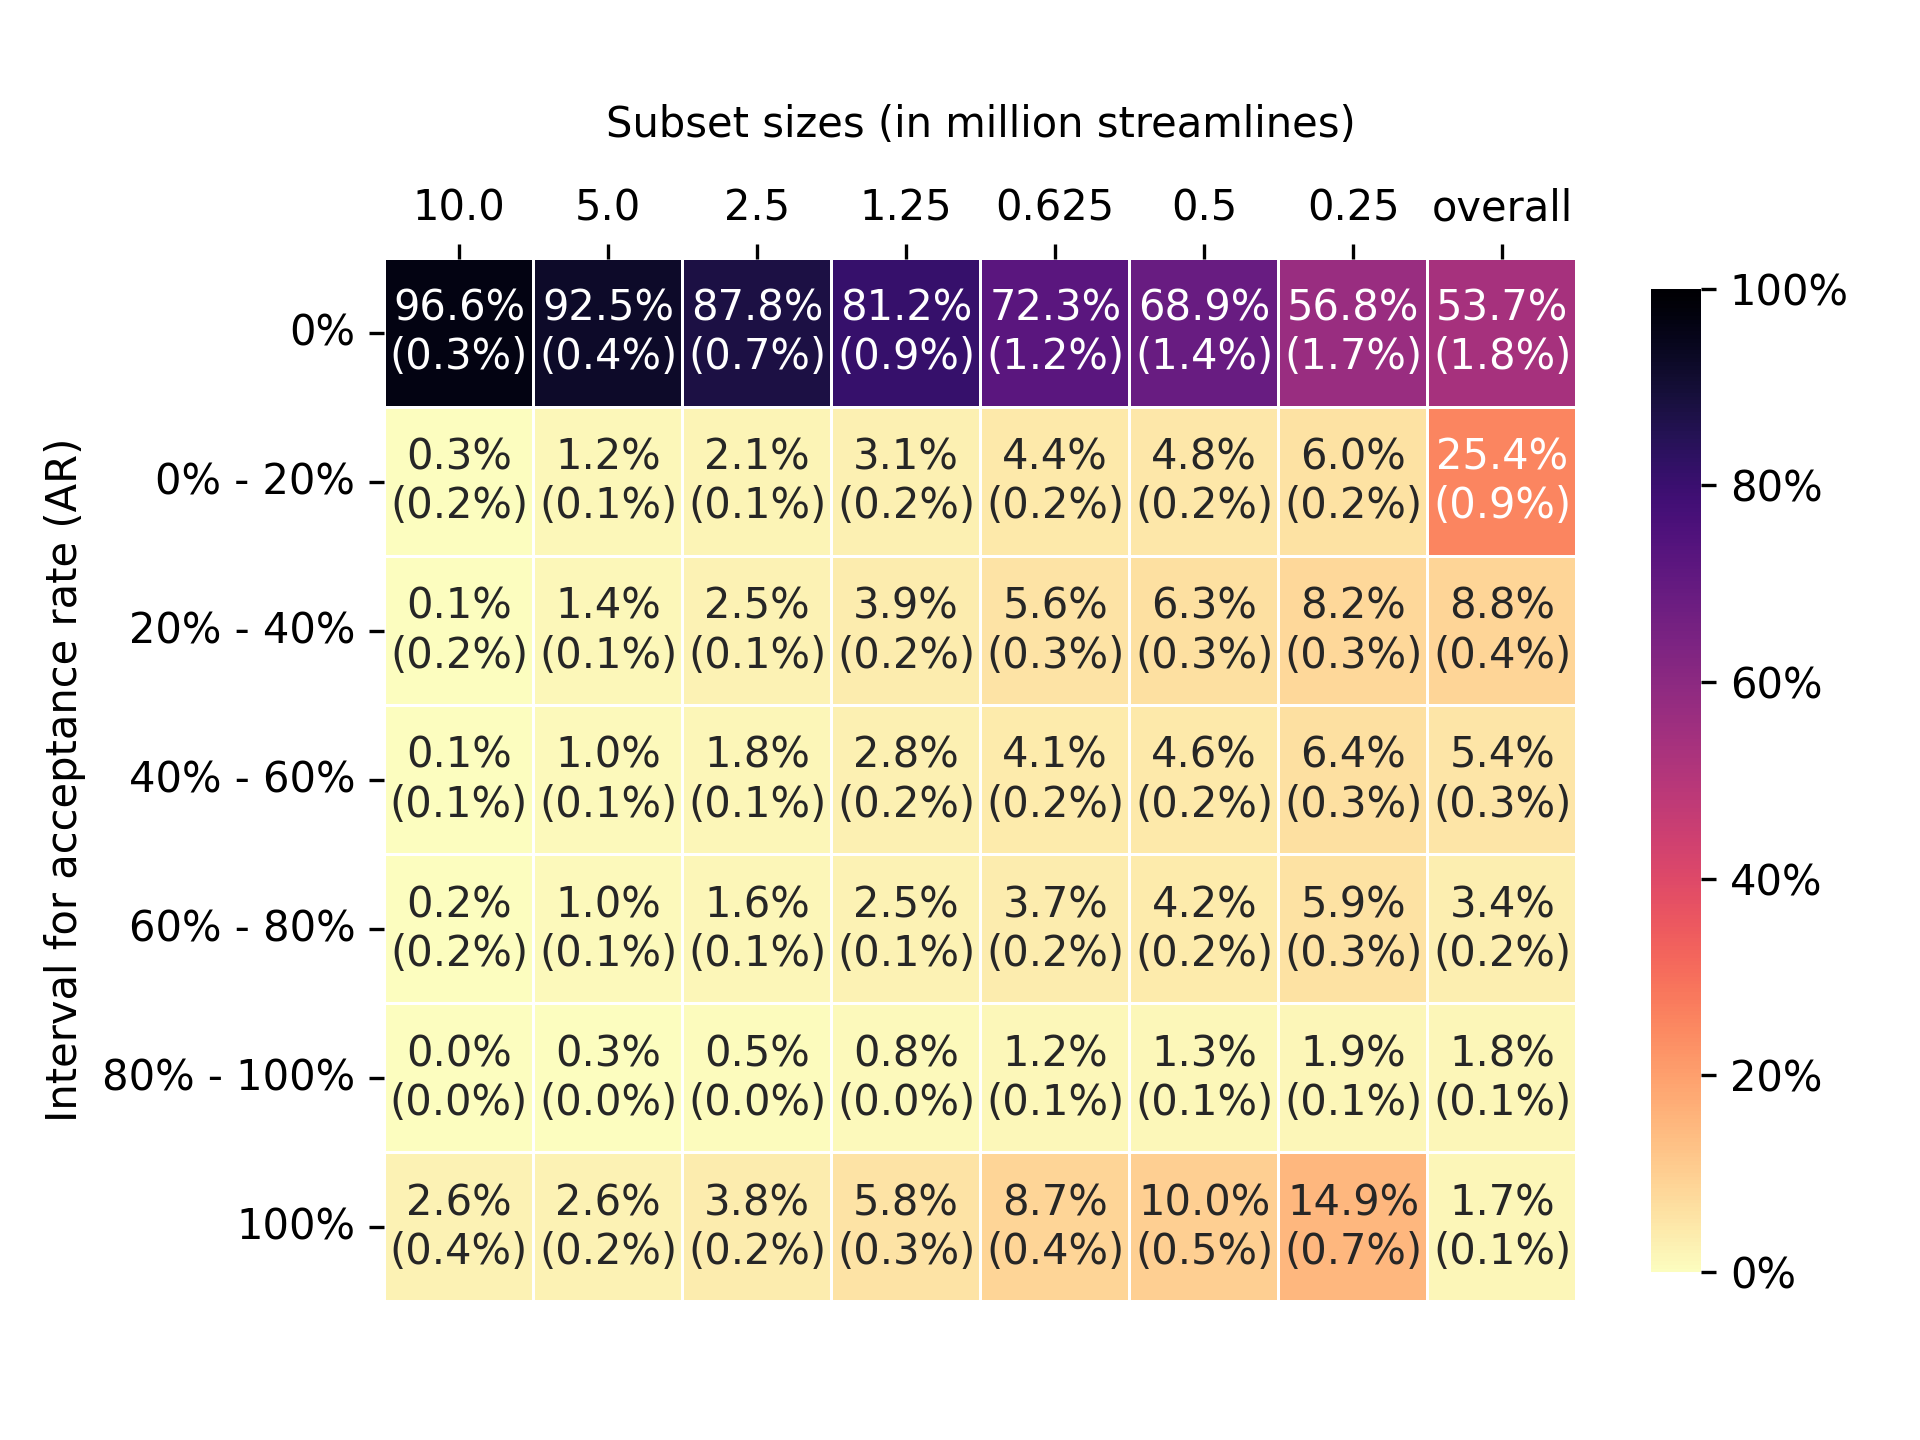
\includegraphics[width= 12cm]{figures/table_rsift.png}
        \caption{The distribution of acceptance rates in different subset sizes in rSIFT \cite{hainAssessingStreamlinePlausibility2022}.
        }
    \label{fig:heatmap_sift}
\end{figure}


Second, the distribution of streamlines of three subjects in different groups are compared in Table \ref*{table:plaus} and \ref*{table:implaus}.
Overall, the scale of implausible groups from both methods is larger than the plausible groups.
In Table \ref*{table:plaus}, the numbers of plausible streamlines extracted by rSIFT are significantly lower than those from rCOMMIT.
While in Table \ref*{table:implaus}, the numbers of implausible streamlines extracted by rSIFT are much higher than those from rCOMMIT.
\begin{table}[!ht]
    \centering
    \caption{The number of streamlines in plausible group of the same subjects between rCOMMIT and rSIFT.}
    ~\\
    \label{table:plaus}
    \begin{tabular}{p{3cm}|p{3cm}|p{3cm}|p{3cm}}
    \toprule
    \multicolumn{4}{c}{\textbf{Plausible Group Between rCOMMIT and rSIFT}} \\
    \toprule
    Subject No. & rCOMMIT & rSIFT & Intersection \\
    \hline
    599967 & 475,959 &146,252 & 89,052 \\
    \hline
    665254 & 215,796 &170,814 & 62,376 \\
    \hline
    837964 & 379,458 &176,320 & 88,175 \\
    \bottomrule
    \end{tabular}
\end{table}

\begin{table}[!ht]
    \centering
    \caption{The number of streamlines in implausible group of the same subjects between rCOMMIT and rSIFT.}
    ~\\
    \label{table:implaus}
    \begin{tabular}{p{3cm}|p{3cm}|p{3cm}|p{3cm}}
    \toprule
    \multicolumn{4}{c}{\textbf{Implausible Group Between rCOMMIT and rSIFT}} \\
    \toprule
    Subject No. & rCOMMIT & rSIFT & Intersection \\
    \hline
    599967 & 1,663,161 &5,263,290 & 1,486,537 \\
    \hline
    665254 & 1,970,751 &5,445,176 & 1,813,401 \\
    \hline
    837964 & 2,581,409 &5,195,768 & 2,215,674 \\
    \bottomrule
    \end{tabular}
\end{table}

Third, with the results from both methods on the same subjects, the comparison on the intersection between two sets of pseudo ground truths
is conducted. The Intersection parts in both plausible and implausible groups indicate a portion of streamlines that obtain the 
same and consistent results from COMMIT and SIFT. The Fig. \ref*{fig:com_s_c} shows the intersection of streamlines from one subjeect in both plausible 
and implausible groups from rCOMMIT and rSIFT. 
The figure on the left represents plausible groups, the values inside the circle are the proportion of each set
according to the original size which is 10 million. Plausible groups in both methods are not big, but the intersection part
takes a significant proportion with the respect to both plausible groups. For the implausible groups, the intersection takes a great amount in both sides. 
And it shows most of the implausible streamlines from rCOMMIT are also recognized by rSIFT as implausible.


\begin{figure}[ht]
    \centering
    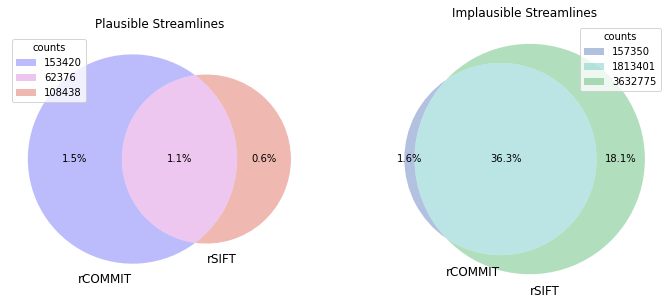
\includegraphics[width= 12cm]{figures/comp_s_c.png}
        \caption{The venn diagrams of the plausible groups and implausible groups from rCOMMIT and rSIFT.}
    \label{fig:com_s_c}
\end{figure}

Last, to investigate the relationship between the distribution and the length of streamlines in rSIFT, an exemplary 
pseudo ground truth from rSIFT is visualized in Fig. \ref*{fig:threegroup_sift}. Similar to the numerical results,
the proportion of implausible streamlines is much higher than the plausible group. Besides, the plausible group is also of lower variety in length.
Unlike rCOMMIT, the proportion of implausible groups seems to largely decrease.

\begin{figure}[ht]
    \centering
    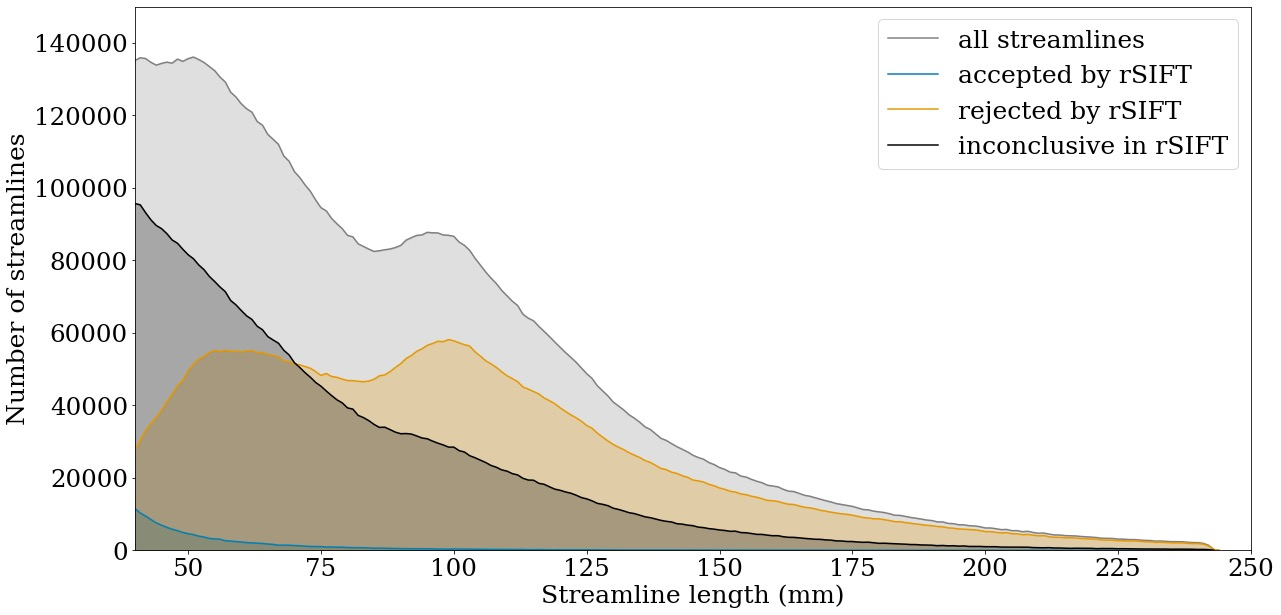
\includegraphics[width= 12cm]{figures/distribution_sift.png}
    \caption{The distribution of streamlines from one exemplary subject after rSIFT \cite{hainAssessingStreamlinePlausibility2022}. }
\label{fig:threegroup_sift}
\end{figure}


\section{Classifier Performance}
Multiple classifiers are applied on the datasets from the experiments. The first part of classification result
is based on the pseudo ground true from rCOMMIT. The second part exploits and combine the dataset 
from both rCOMMIT and rSIFT.
\subsection{Performance based on rCOMMIT}

An overview of the classifier performance is shown in Fig.

\begin{figure}[ht]
    \centering
    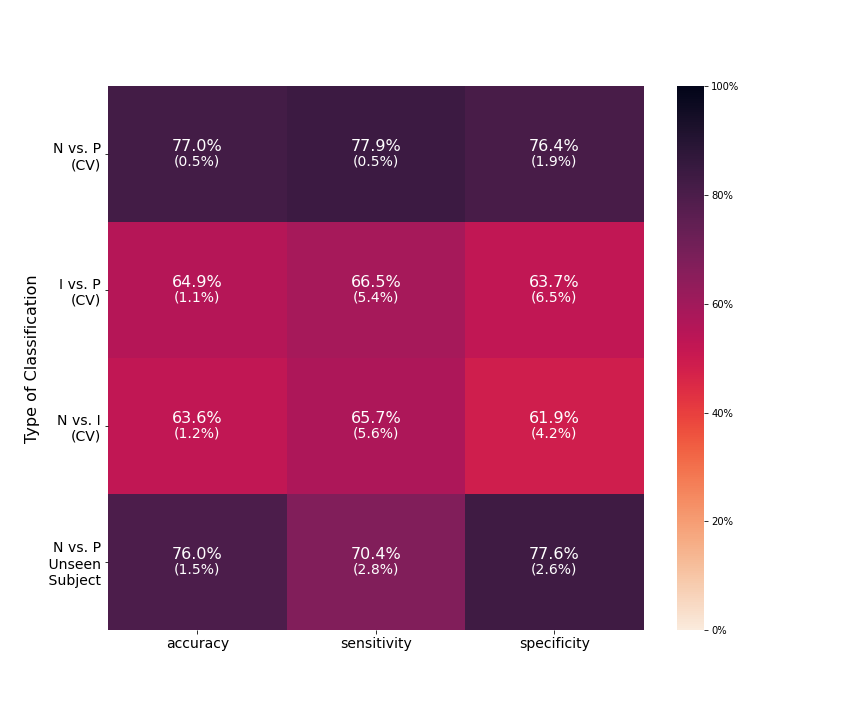
\includegraphics[width= 12cm]{figures/rcommit_classifiers.png}
    \caption{The performance of binary classifiers based on the pseudo ground truth from rCOMMIT.
    “P” represents “positive” (plausible),  “N” represents “negative” (implausible), and “I” inconclusive. 
    The metrics are computed through the mean values as determined by 3-fold cross-validation (CV) in training or tests with the unseen subject during training, 
    with standard deviations in parentheses.}
\label{fig:rcommit_classifiers}
\end{figure}


\begin{figure}[ht]
    \centering
    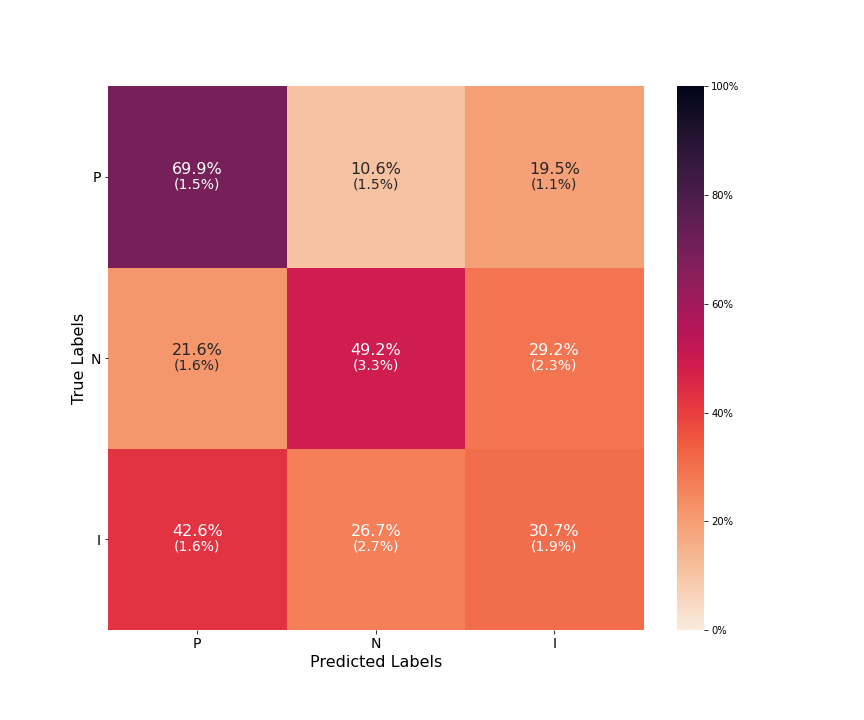
\includegraphics[width= 12cm]{figures/multi_class.png}
    \caption{The performance of multi-class classifiers based on the pseudo ground truth from rCOMMIT.
    }
\label{fig:rcommit_multi_classifiers}
\end{figure}

\begin{figure}[ht]
    \centering
    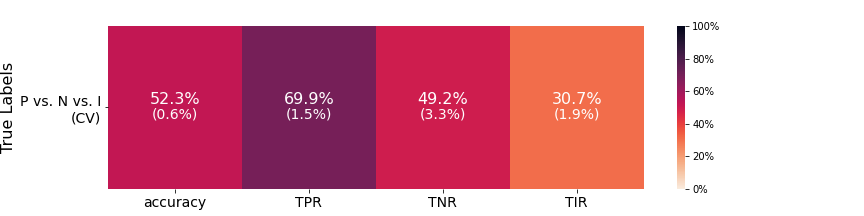
\includegraphics[width= 12cm]{figures/multi_class_critiaria.png}
    \caption{The performance of multi-class classifiers based on the pseudo ground truth from rCOMMIT.
    }
\label{fig:multi_classifiers_critiaria}
\end{figure}


\subsection{Performance based on the intersection between rCOMMIT and rSIFT}
With the pseudo ground truths from both rCOMMIT and rSIFT, the intersection of both data is extracted and used as the new training data.
An overview of the performance of the binary classifiers trained on it is shown in Fig. \ref{fig:inter_classifiers}.
The accuracy of binary classifiers on plausible and implausible streamlines is higher than the accuracy of rCOMMIT binary classifiers.
Meanwhile, the accuracy of the classifiers on plausible and inconclusive streamlines also increases.

\begin{figure}[ht]
    \centering
    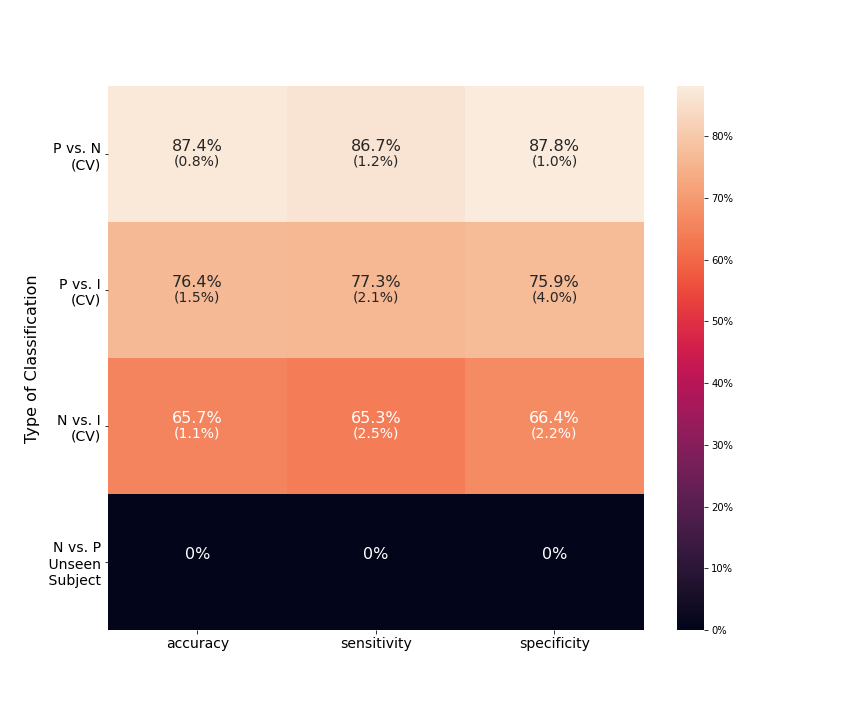
\includegraphics[width= 12cm]{figures/inter_classifiers.png}
    \caption{The performance of binary classifiers based on the intersection data from rCOMMIT and rSIFT.
    “P” represents “positive” (plausible),  “N” represents “negative” (implausible), and “I” inconclusive. 
    The metrics are computed through the mean values as determined by 5-fold cross-validation (CV) in training or tests with unseen subjects during training, 
    with standard deviations in parentheses.}
\label{fig:inter_classifiers}
\end{figure}
